\documentclass[twoside]{book}

% Packages required by doxygen
\usepackage{fixltx2e}
\usepackage{calc}
\usepackage{doxygen}
\usepackage[export]{adjustbox} % also loads graphicx
\usepackage{graphicx}
\usepackage[utf8]{inputenc}
\usepackage{makeidx}
\usepackage{multicol}
\usepackage{multirow}
\PassOptionsToPackage{warn}{textcomp}
\usepackage{textcomp}
\usepackage[nointegrals]{wasysym}
\usepackage[table]{xcolor}

% Font selection
\usepackage[T1]{fontenc}
\usepackage[scaled=.90]{helvet}
\usepackage{courier}
\usepackage{amssymb}
\usepackage{sectsty}
\renewcommand{\familydefault}{\sfdefault}
\allsectionsfont{%
  \fontseries{bc}\selectfont%
  \color{darkgray}%
}
\renewcommand{\DoxyLabelFont}{%
  \fontseries{bc}\selectfont%
  \color{darkgray}%
}
\newcommand{\+}{\discretionary{\mbox{\scriptsize$\hookleftarrow$}}{}{}}

% Page & text layout
\usepackage{geometry}
\geometry{%
  a4paper,%
  top=2.5cm,%
  bottom=2.5cm,%
  left=2.5cm,%
  right=2.5cm%
}
\tolerance=750
\hfuzz=15pt
\hbadness=750
\setlength{\emergencystretch}{15pt}
\setlength{\parindent}{0cm}
\setlength{\parskip}{3ex plus 2ex minus 2ex}
\makeatletter
\renewcommand{\paragraph}{%
  \@startsection{paragraph}{4}{0ex}{-1.0ex}{1.0ex}{%
    \normalfont\normalsize\bfseries\SS@parafont%
  }%
}
\renewcommand{\subparagraph}{%
  \@startsection{subparagraph}{5}{0ex}{-1.0ex}{1.0ex}{%
    \normalfont\normalsize\bfseries\SS@subparafont%
  }%
}
\makeatother

% Headers & footers
\usepackage{fancyhdr}
\pagestyle{fancyplain}
\fancyhead[LE]{\fancyplain{}{\bfseries\thepage}}
\fancyhead[CE]{\fancyplain{}{}}
\fancyhead[RE]{\fancyplain{}{\bfseries\leftmark}}
\fancyhead[LO]{\fancyplain{}{\bfseries\rightmark}}
\fancyhead[CO]{\fancyplain{}{}}
\fancyhead[RO]{\fancyplain{}{\bfseries\thepage}}
\fancyfoot[LE]{\fancyplain{}{}}
\fancyfoot[CE]{\fancyplain{}{}}
\fancyfoot[RE]{\fancyplain{}{\bfseries\scriptsize Generated by Doxygen }}
\fancyfoot[LO]{\fancyplain{}{\bfseries\scriptsize Generated by Doxygen }}
\fancyfoot[CO]{\fancyplain{}{}}
\fancyfoot[RO]{\fancyplain{}{}}
\renewcommand{\footrulewidth}{0.4pt}
\renewcommand{\chaptermark}[1]{%
  \markboth{#1}{}%
}
\renewcommand{\sectionmark}[1]{%
  \markright{\thesection\ #1}%
}

% Indices & bibliography
\usepackage{natbib}
\usepackage[titles]{tocloft}
\setcounter{tocdepth}{3}
\setcounter{secnumdepth}{5}
\makeindex

% Hyperlinks (required, but should be loaded last)
\usepackage{ifpdf}
\ifpdf
  \usepackage[pdftex,pagebackref=true]{hyperref}
\else
  \usepackage[ps2pdf,pagebackref=true]{hyperref}
\fi
\hypersetup{%
  colorlinks=true,%
  linkcolor=blue,%
  citecolor=blue,%
  unicode%
}

% Custom commands
\newcommand{\clearemptydoublepage}{%
  \newpage{\pagestyle{empty}\cleardoublepage}%
}

\usepackage{caption}
\captionsetup{labelsep=space,justification=centering,font={bf},singlelinecheck=off,skip=4pt,position=top}

%===== C O N T E N T S =====

\begin{document}

% Titlepage & ToC
\hypersetup{pageanchor=false,
             bookmarksnumbered=true,
             pdfencoding=unicode
            }
\pagenumbering{alph}
\begin{titlepage}
\vspace*{7cm}
\begin{center}%
{\Large Triad \\[1ex]\large 0.\+1 }\\
\vspace*{1cm}
{\large Generated by Doxygen 1.8.13}\\
\end{center}
\end{titlepage}
\clearemptydoublepage
\pagenumbering{roman}
\tableofcontents
\clearemptydoublepage
\pagenumbering{arabic}
\hypersetup{pageanchor=true}

%--- Begin generated contents ---
\chapter{Hierarchical Index}
\section{Class Hierarchy}
This inheritance list is sorted roughly, but not completely, alphabetically\+:\begin{DoxyCompactList}
\item \contentsline{section}{Dom\+Item}{\pageref{classDomItem}}{}
\item Q\+Abstract\+Item\+Model\begin{DoxyCompactList}
\item \contentsline{section}{Note\+Model}{\pageref{classNoteModel}}{}
\end{DoxyCompactList}
\item Q\+Object\begin{DoxyCompactList}
\item \contentsline{section}{Access}{\pageref{classAccess}}{}
\item \contentsline{section}{Document\+Handler}{\pageref{classDocumentHandler}}{}
\item \contentsline{section}{Image\+Base\+Converter}{\pageref{classImageBaseConverter}}{}
\item \contentsline{section}{Storage\+Interface}{\pageref{classStorageInterface}}{}
\end{DoxyCompactList}
\end{DoxyCompactList}

\chapter{Class Index}
\section{Class List}
Here are the classes, structs, unions and interfaces with brief descriptions\+:\begin{DoxyCompactList}
\item\contentsline{section}{\hyperlink{classDocumentHandler}{Document\+Handler} }{\pageref{classDocumentHandler}}{}
\item\contentsline{section}{\hyperlink{classDomItem}{Dom\+Item} }{\pageref{classDomItem}}{}
\item\contentsline{section}{\hyperlink{classImageBaseConverter}{Image\+Base\+Converter} }{\pageref{classImageBaseConverter}}{}
\item\contentsline{section}{\hyperlink{classNoteModel}{Note\+Model} }{\pageref{classNoteModel}}{}
\item\contentsline{section}{\hyperlink{classStorageInterface}{Storage\+Interface} \\*Acts as a liason between the model and the UI }{\pageref{classStorageInterface}}{}
\end{DoxyCompactList}

\chapter{Class Documentation}
\hypertarget{classDocumentHandler}{}\section{Document\+Handler Class Reference}
\label{classDocumentHandler}\index{Document\+Handler@{Document\+Handler}}
Inheritance diagram for Document\+Handler\+:\begin{figure}[H]
\begin{center}
\leavevmode
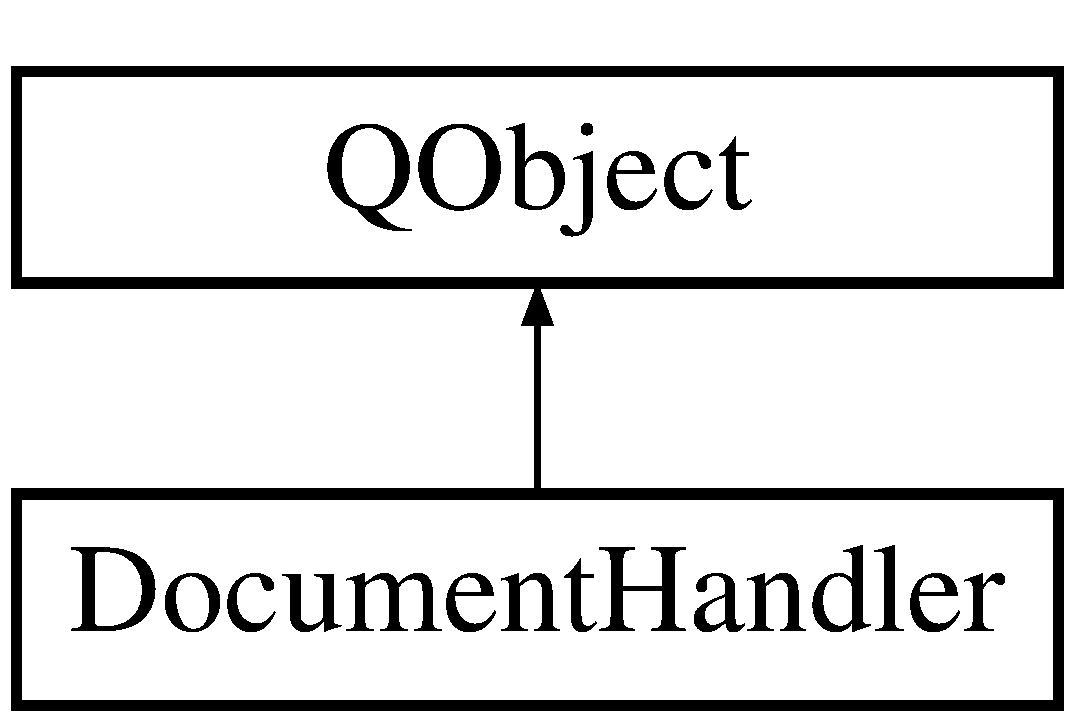
\includegraphics[height=2.000000cm]{classDocumentHandler}
\end{center}
\end{figure}
\subsection*{Public Slots}
\begin{DoxyCompactItemize}
\item 
\mbox{\Hypertarget{classDocumentHandler_a0ecd6f194d033839ad435774a9e69175}\label{classDocumentHandler_a0ecd6f194d033839ad435774a9e69175}} 
void {\bfseries change} ()
\end{DoxyCompactItemize}
\subsection*{Public Member Functions}
\begin{DoxyCompactItemize}
\item 
\mbox{\Hypertarget{classDocumentHandler_abf07f38e288c50a5b154c776e75d8ba7}\label{classDocumentHandler_abf07f38e288c50a5b154c776e75d8ba7}} 
{\bfseries Document\+Handler} (Q\+Object $\ast$parent=nullptr)
\item 
\mbox{\Hypertarget{classDocumentHandler_a7d6d1a0cbcc8eb6fcd3f84d2dd082504}\label{classDocumentHandler_a7d6d1a0cbcc8eb6fcd3f84d2dd082504}} 
void {\bfseries set\+Text\+Document} (Q\+Quick\+Text\+Document $\ast$textdoc)
\item 
\mbox{\Hypertarget{classDocumentHandler_a0cd35353f607043bec0e2e5d9da2fd60}\label{classDocumentHandler_a0cd35353f607043bec0e2e5d9da2fd60}} 
Q\+Quick\+Text\+Document $\ast$ {\bfseries get\+Text\+Document} ()
\item 
\mbox{\Hypertarget{classDocumentHandler_aa3ab0c2553bccd2bfea3463cd133b7a4}\label{classDocumentHandler_aa3ab0c2553bccd2bfea3463cd133b7a4}} 
void {\bfseries set\+Node} (Q\+Variant node)
\item 
\mbox{\Hypertarget{classDocumentHandler_acd199a4ee29b54c1d23d1046cd2961f0}\label{classDocumentHandler_acd199a4ee29b54c1d23d1046cd2961f0}} 
Q\+Variant {\bfseries get\+Node} ()
\item 
\mbox{\Hypertarget{classDocumentHandler_a1c107f1f558d56fa8164c7eac47f0411}\label{classDocumentHandler_a1c107f1f558d56fa8164c7eac47f0411}} 
double {\bfseries get\+X\+Pos} ()
\item 
\mbox{\Hypertarget{classDocumentHandler_a49dd035721a4252b2930cfa49b53b0d2}\label{classDocumentHandler_a49dd035721a4252b2930cfa49b53b0d2}} 
void {\bfseries set\+X\+Pos} (double xpos)
\item 
\mbox{\Hypertarget{classDocumentHandler_a327788c6a3d111e4f8c4b040cde17a78}\label{classDocumentHandler_a327788c6a3d111e4f8c4b040cde17a78}} 
double {\bfseries get\+Y\+Pos} ()
\item 
\mbox{\Hypertarget{classDocumentHandler_ad6f687b5df8747329d5885cd43243374}\label{classDocumentHandler_ad6f687b5df8747329d5885cd43243374}} 
void {\bfseries set\+Y\+Pos} (double ypos)
\end{DoxyCompactItemize}
\subsection*{Properties}
\begin{DoxyCompactItemize}
\item 
\mbox{\Hypertarget{classDocumentHandler_af2cc4935d7d4c0c358a9ce92402a2713}\label{classDocumentHandler_af2cc4935d7d4c0c358a9ce92402a2713}} 
Q\+Quick\+Text\+Document {\bfseries text\+Document}
\item 
\mbox{\Hypertarget{classDocumentHandler_a76d9b652387d682951cccf452a76ea90}\label{classDocumentHandler_a76d9b652387d682951cccf452a76ea90}} 
Q\+Variant {\bfseries node}
\item 
\mbox{\Hypertarget{classDocumentHandler_a0f3b97be34c7e4a3e47635ba65cddb9a}\label{classDocumentHandler_a0f3b97be34c7e4a3e47635ba65cddb9a}} 
double {\bfseries xpos}
\item 
\mbox{\Hypertarget{classDocumentHandler_a3e7cfabf2b8c55e97572a19848e05b52}\label{classDocumentHandler_a3e7cfabf2b8c55e97572a19848e05b52}} 
double {\bfseries ypos}
\end{DoxyCompactItemize}


\subsection{Detailed Description}


Definition at line 11 of file documenthandler.\+h.



The documentation for this class was generated from the following files\+:\begin{DoxyCompactItemize}
\item 
includes/documenthandler.\+h\item 
src/documenthandler.\+cpp\end{DoxyCompactItemize}

\hypertarget{classDomItem}{}\section{Dom\+Item Class Reference}
\label{classDomItem}\index{Dom\+Item@{Dom\+Item}}
\subsection*{Public Member Functions}
\begin{DoxyCompactItemize}
\item 
\mbox{\Hypertarget{classDomItem_ab7b614325927474e2ffe492984b0ba93}\label{classDomItem_ab7b614325927474e2ffe492984b0ba93}} 
{\bfseries Dom\+Item} (Q\+Dom\+Node \&\hyperlink{classDomItem_a29a7202350961e4640a895ebc1daf3a0}{node}, int \hyperlink{classDomItem_ad08a9979184909d70fb2f5000dd5a7b9}{row}, \hyperlink{classDomItem}{Dom\+Item} $\ast$\hyperlink{classDomItem_abba8216c2555c524a9ac662834019c30}{parent}=0)
\item 
\hyperlink{classDomItem}{Dom\+Item} $\ast$ \hyperlink{classDomItem_af1f0d64a01b07fce3d310fe71da81ca7}{child} (int i)
\begin{DoxyCompactList}\small\item\em child accesses a contained \hyperlink{classDomItem}{Dom\+Item} represented by i. \end{DoxyCompactList}\item 
\mbox{\Hypertarget{classDomItem_a30a370dc17a163568065288050ce2c37}\label{classDomItem_a30a370dc17a163568065288050ce2c37}} 
\hyperlink{classDomItem}{Dom\+Item} $\ast$ {\bfseries child} ()
\item 
\mbox{\Hypertarget{classDomItem_abba8216c2555c524a9ac662834019c30}\label{classDomItem_abba8216c2555c524a9ac662834019c30}} 
\hyperlink{classDomItem}{Dom\+Item} $\ast$ \hyperlink{classDomItem_abba8216c2555c524a9ac662834019c30}{parent} ()
\begin{DoxyCompactList}\small\item\em Convenience function to access the first child \hyperlink{classDomItem}{Dom\+Item}. \end{DoxyCompactList}\item 
\mbox{\Hypertarget{classDomItem_a29a7202350961e4640a895ebc1daf3a0}\label{classDomItem_a29a7202350961e4640a895ebc1daf3a0}} 
Q\+Dom\+Node \hyperlink{classDomItem_a29a7202350961e4640a895ebc1daf3a0}{node} () const
\begin{DoxyCompactList}\small\item\em Returns the parent \hyperlink{classDomItem}{Dom\+Item}. \end{DoxyCompactList}\item 
\mbox{\Hypertarget{classDomItem_ad08a9979184909d70fb2f5000dd5a7b9}\label{classDomItem_ad08a9979184909d70fb2f5000dd5a7b9}} 
int \hyperlink{classDomItem_ad08a9979184909d70fb2f5000dd5a7b9}{row} ()
\begin{DoxyCompactList}\small\item\em Returns the internal Q\+Dom\+Node that \hyperlink{classDomItem}{Dom\+Item} wraps. \end{DoxyCompactList}\end{DoxyCompactItemize}


\subsection{Detailed Description}


Definition at line 60 of file domitem.\+h.



\subsection{Member Function Documentation}
\mbox{\Hypertarget{classDomItem_af1f0d64a01b07fce3d310fe71da81ca7}\label{classDomItem_af1f0d64a01b07fce3d310fe71da81ca7}} 
\index{Dom\+Item@{Dom\+Item}!child@{child}}
\index{child@{child}!Dom\+Item@{Dom\+Item}}
\subsubsection{\texorpdfstring{child()}{child()}}
{\footnotesize\ttfamily \hyperlink{classDomItem}{Dom\+Item} $\ast$ Dom\+Item\+::child (\begin{DoxyParamCaption}\item[{int}]{i }\end{DoxyParamCaption})}



child accesses a contained \hyperlink{classDomItem}{Dom\+Item} represented by i. 


\begin{DoxyParams}{Parameters}
{\em i} & The index of the desired child \hyperlink{classDomItem}{Dom\+Item} \\
\hline
\end{DoxyParams}
\begin{DoxyReturn}{Returns}
a \hyperlink{classDomItem}{Dom\+Item}
\end{DoxyReturn}
This function accesses a child \hyperlink{classDomItem}{Dom\+Item} corresponding to the index i. If no \hyperlink{classDomItem}{Dom\+Item} exists corresponding to that index, it tries to create one from a Q\+Dom\+Node in the underlying Q\+Dom\+Document structure. 

Definition at line 83 of file domitem.\+cpp.



The documentation for this class was generated from the following files\+:\begin{DoxyCompactItemize}
\item 
includes/domitem.\+h\item 
src/domitem.\+cpp\end{DoxyCompactItemize}

\hypertarget{classImageBaseConverter}{}\section{Image\+Base\+Converter Class Reference}
\label{classImageBaseConverter}\index{Image\+Base\+Converter@{Image\+Base\+Converter}}
Inheritance diagram for Image\+Base\+Converter\+:\begin{figure}[H]
\begin{center}
\leavevmode
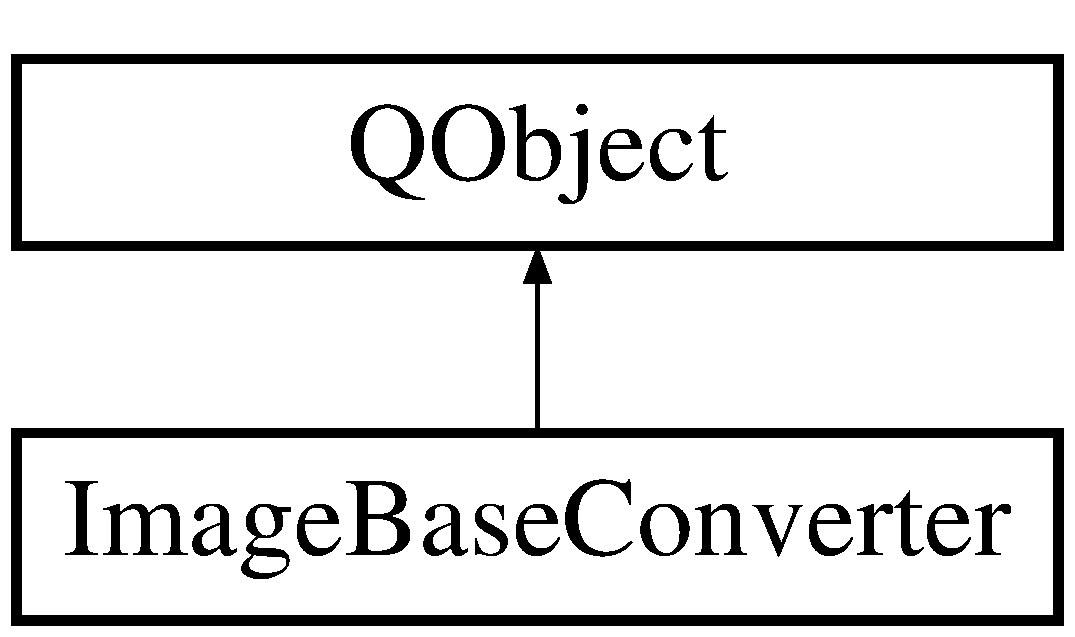
\includegraphics[height=2.000000cm]{classImageBaseConverter}
\end{center}
\end{figure}
\subsection*{Public Member Functions}
\begin{DoxyCompactItemize}
\item 
\mbox{\Hypertarget{classImageBaseConverter_ad5a3543b251a7395d73a8888ab1baa00}\label{classImageBaseConverter_ad5a3543b251a7395d73a8888ab1baa00}} 
{\bfseries Image\+Base\+Converter} (Q\+Object $\ast$parent=nullptr)
\item 
\mbox{\Hypertarget{classImageBaseConverter_a01ed6b49c6d050860c84c07fb894be62}\label{classImageBaseConverter_a01ed6b49c6d050860c84c07fb894be62}} 
Q\+\_\+\+I\+N\+V\+O\+K\+A\+B\+LE Q\+String {\bfseries gen} (Q\+String path)
\end{DoxyCompactItemize}


\subsection{Detailed Description}


Definition at line 6 of file imagebaseconverter.\+h.



The documentation for this class was generated from the following files\+:\begin{DoxyCompactItemize}
\item 
includes/imagebaseconverter.\+h\item 
src/imagebaseconverter.\+cpp\end{DoxyCompactItemize}

\hypertarget{classNoteModel}{}\section{Note\+Model Class Reference}
\label{classNoteModel}\index{Note\+Model@{Note\+Model}}
Inheritance diagram for Note\+Model\+:\begin{figure}[H]
\begin{center}
\leavevmode
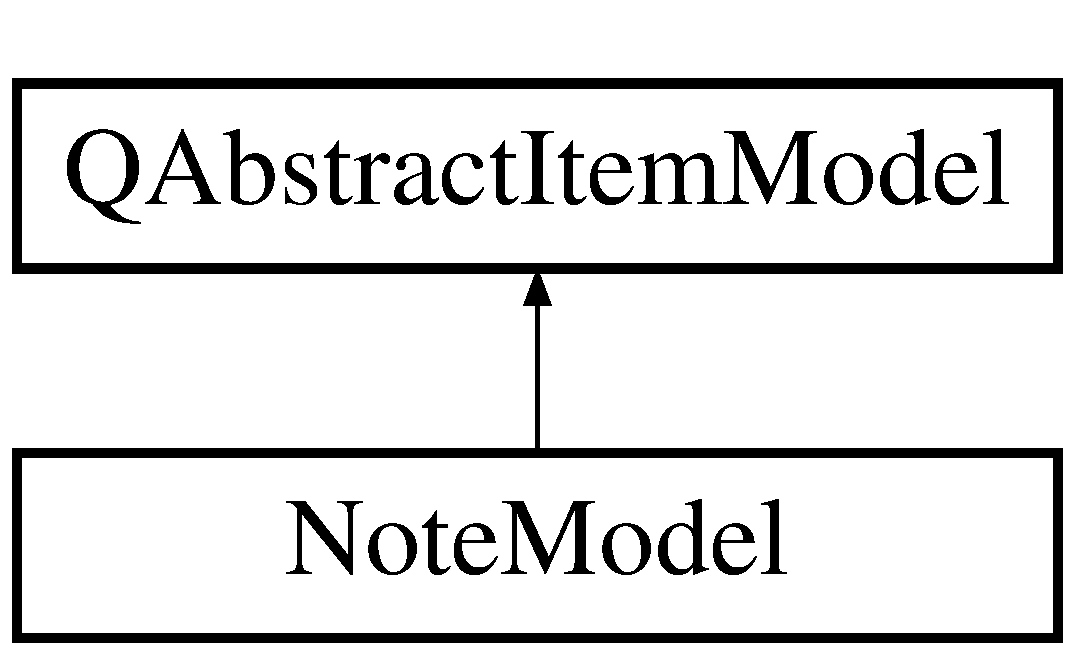
\includegraphics[height=2.000000cm]{classNoteModel}
\end{center}
\end{figure}
\subsection*{Public Types}
\begin{DoxyCompactItemize}
\item 
\mbox{\Hypertarget{classNoteModel_a77008f4402a891e33a05e4bd603d0fc3}\label{classNoteModel_a77008f4402a891e33a05e4bd603d0fc3}} 
enum {\bfseries Note\+Model\+Roles} \{ {\bfseries Title} = Qt\+:\+:User\+Role, 
{\bfseries Content}
 \}
\end{DoxyCompactItemize}
\subsection*{Public Member Functions}
\begin{DoxyCompactItemize}
\item 
\mbox{\Hypertarget{classNoteModel_a8cdb8b7c9a4a7230b6703593b9881a38}\label{classNoteModel_a8cdb8b7c9a4a7230b6703593b9881a38}} 
{\bfseries Note\+Model} (Q\+Object $\ast$parent=nullptr)
\item 
\mbox{\Hypertarget{classNoteModel_a5c2b327f4aceca68ce84627dd14d3eed}\label{classNoteModel_a5c2b327f4aceca68ce84627dd14d3eed}} 
Qt\+::\+Item\+Flags {\bfseries flags} (const Q\+Model\+Index \&index) const override
\item 
\mbox{\Hypertarget{classNoteModel_af7b59b219ab71617116f6dd74f315766}\label{classNoteModel_af7b59b219ab71617116f6dd74f315766}} 
Q\+Variant {\bfseries data} (const Q\+Model\+Index \&index, int role=Qt\+::\+Display\+Role) const override
\item 
\mbox{\Hypertarget{classNoteModel_a94ede21a096dba8a182efe70a6235ff8}\label{classNoteModel_a94ede21a096dba8a182efe70a6235ff8}} 
Q\+Variant {\bfseries header\+Data} (int section, Qt\+::\+Orientation orientation, int role=Qt\+::\+Display\+Role) const override
\item 
\mbox{\Hypertarget{classNoteModel_a0c569f32aa87c740fb2d646c54e5334d}\label{classNoteModel_a0c569f32aa87c740fb2d646c54e5334d}} 
Q\+Model\+Index {\bfseries index} (int row, int column, const Q\+Model\+Index \&parent=Q\+Model\+Index()) const override
\item 
\mbox{\Hypertarget{classNoteModel_a2ee27f84cd8fe9b0e7f0222bace1fb7f}\label{classNoteModel_a2ee27f84cd8fe9b0e7f0222bace1fb7f}} 
Q\+Model\+Index {\bfseries parent} (const Q\+Model\+Index \&child) const override
\item 
\mbox{\Hypertarget{classNoteModel_af46fc83db7101b3e332382b0804ef51b}\label{classNoteModel_af46fc83db7101b3e332382b0804ef51b}} 
Q\+Hash$<$ int, Q\+Byte\+Array $>$ {\bfseries role\+Names} () const override
\item 
\mbox{\Hypertarget{classNoteModel_a1abbcfea2189d4496ddb25332a73ab38}\label{classNoteModel_a1abbcfea2189d4496ddb25332a73ab38}} 
int {\bfseries row\+Count} (const Q\+Model\+Index \&parent=Q\+Model\+Index()) const override
\item 
\mbox{\Hypertarget{classNoteModel_ada056af2d7b7ff4ab515e9f01867aae6}\label{classNoteModel_ada056af2d7b7ff4ab515e9f01867aae6}} 
int {\bfseries column\+Count} (const Q\+Model\+Index \&parent=Q\+Model\+Index()) const override
\end{DoxyCompactItemize}


\subsection{Detailed Description}


Definition at line 62 of file notemodel.\+h.



The documentation for this class was generated from the following files\+:\begin{DoxyCompactItemize}
\item 
includes/notemodel.\+h\item 
src/notemodel.\+cpp\end{DoxyCompactItemize}

\hypertarget{classStorageInterface}{}\section{Storage\+Interface Class Reference}
\label{classStorageInterface}\index{Storage\+Interface@{Storage\+Interface}}


The \hyperlink{classStorageInterface}{Storage\+Interface} class acts as a liason between the model and the UI.  




{\ttfamily \#include $<$storageinterface.\+h$>$}

Inheritance diagram for Storage\+Interface\+:\begin{figure}[H]
\begin{center}
\leavevmode
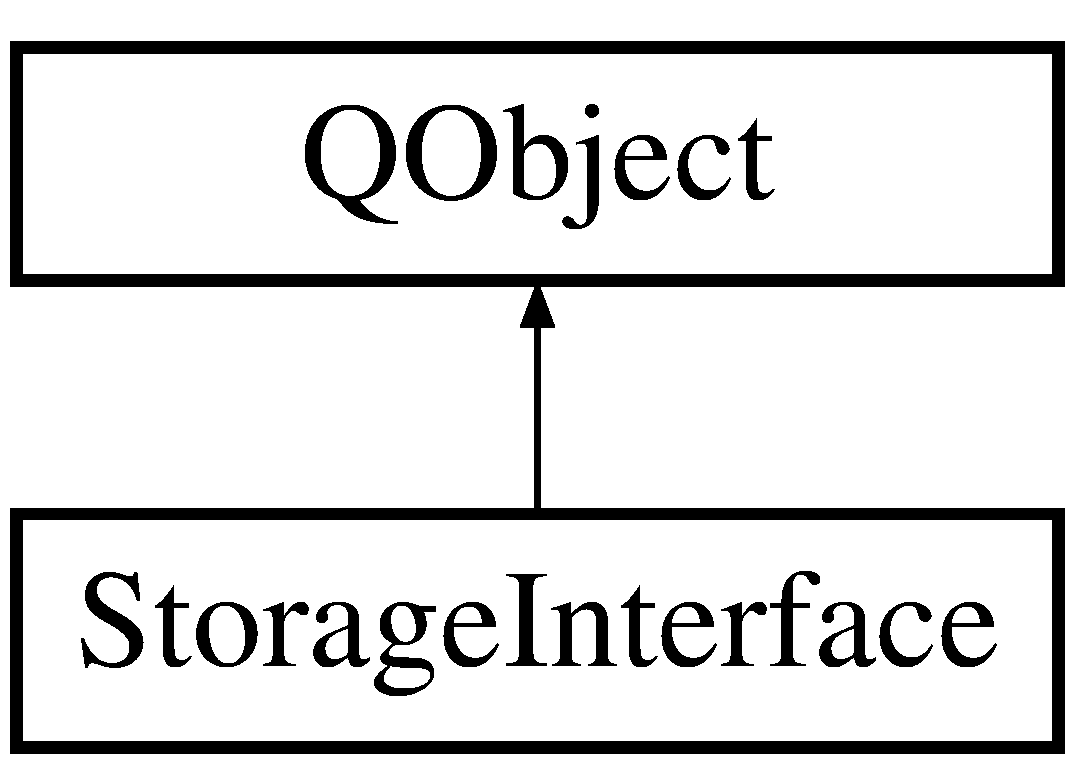
\includegraphics[height=2.000000cm]{classStorageInterface}
\end{center}
\end{figure}
\subsection*{Public Slots}
\begin{DoxyCompactItemize}
\item 
\mbox{\Hypertarget{classStorageInterface_a92a1fdb2cb4576b31fa236f8e2020f73}\label{classStorageInterface_a92a1fdb2cb4576b31fa236f8e2020f73}} 
Q\+Variant {\bfseries create\+Node} ()
\item 
\mbox{\Hypertarget{classStorageInterface_a48970a8eb1a4ddba216df0f628f48347}\label{classStorageInterface_a48970a8eb1a4ddba216df0f628f48347}} 
Q\+Variant {\bfseries pop\+Element} ()
\item 
\mbox{\Hypertarget{classStorageInterface_aaa04b04a58411bbb50cff07b6d4b2d21}\label{classStorageInterface_aaa04b04a58411bbb50cff07b6d4b2d21}} 
void {\bfseries finish\+Loading} ()
\end{DoxyCompactItemize}
\subsection*{Signals}
\begin{DoxyCompactItemize}
\item 
\mbox{\Hypertarget{classStorageInterface_adab2ae35804274ef3773e27757081ffa}\label{classStorageInterface_adab2ae35804274ef3773e27757081ffa}} 
void {\bfseries containers\+Loaded} (int number\+Of\+Loaded\+Elements)
\item 
\mbox{\Hypertarget{classStorageInterface_a34510ab0d18c65460d2f48de9899627a}\label{classStorageInterface_a34510ab0d18c65460d2f48de9899627a}} 
void {\bfseries id\+Changed} (int id)
\end{DoxyCompactItemize}
\subsection*{Public Member Functions}
\begin{DoxyCompactItemize}
\item 
\mbox{\Hypertarget{classStorageInterface_a7586bb58eb326e9746e56762dc1e274e}\label{classStorageInterface_a7586bb58eb326e9746e56762dc1e274e}} 
{\bfseries Storage\+Interface} (Q\+Object $\ast$parent=nullptr)
\item 
\mbox{\Hypertarget{classStorageInterface_ad603f4c3282cbf80bbf4bba5fbd27ad3}\label{classStorageInterface_ad603f4c3282cbf80bbf4bba5fbd27ad3}} 
Q\+\_\+\+I\+N\+V\+O\+K\+A\+B\+LE void {\bfseries save\+Doc} ()
\item 
\mbox{\Hypertarget{classStorageInterface_a51d75b4fdc7fdf2cbbe4c6c8e9963531}\label{classStorageInterface_a51d75b4fdc7fdf2cbbe4c6c8e9963531}} 
Q\+\_\+\+I\+N\+V\+O\+K\+A\+B\+LE double {\bfseries top\+X\+Pos} ()
\item 
\mbox{\Hypertarget{classStorageInterface_a101e97200cce19b0171255139ddc347c}\label{classStorageInterface_a101e97200cce19b0171255139ddc347c}} 
Q\+\_\+\+I\+N\+V\+O\+K\+A\+B\+LE double {\bfseries top\+Y\+Pos} ()
\item 
\mbox{\Hypertarget{classStorageInterface_ad41bc8b449de097657e361762cc38ba2}\label{classStorageInterface_ad41bc8b449de097657e361762cc38ba2}} 
Q\+\_\+\+I\+N\+V\+O\+K\+A\+B\+LE Q\+String {\bfseries top\+Contents} ()
\item 
\mbox{\Hypertarget{classStorageInterface_a0688904dc97ecb5f1693633744e7d065}\label{classStorageInterface_a0688904dc97ecb5f1693633744e7d065}} 
Q\+\_\+\+I\+N\+V\+O\+K\+A\+B\+LE void {\bfseries purge\+Element} (Q\+Variant qdomelement)
\item 
\mbox{\Hypertarget{classStorageInterface_a1616fb52651a1aa8b56431ac91f65b40}\label{classStorageInterface_a1616fb52651a1aa8b56431ac91f65b40}} 
Q\+\_\+\+I\+N\+V\+O\+K\+A\+B\+LE void {\bfseries set\+Content} (int index, Q\+String contents\+String)
\item 
\mbox{\Hypertarget{classStorageInterface_a27e8bcbd40aaa6fd224eff3e9a667499}\label{classStorageInterface_a27e8bcbd40aaa6fd224eff3e9a667499}} 
Q\+\_\+\+I\+N\+V\+O\+K\+A\+B\+LE void {\bfseries set\+X\+Pos} (int index, double x\+\_\+\+Pos)
\item 
\mbox{\Hypertarget{classStorageInterface_a5e517d8704b5ffb89c819e0dd5145fe3}\label{classStorageInterface_a5e517d8704b5ffb89c819e0dd5145fe3}} 
Q\+\_\+\+I\+N\+V\+O\+K\+A\+B\+LE void {\bfseries set\+Y\+Pos} (int index, double y\+\_\+\+Pos)
\item 
\mbox{\Hypertarget{classStorageInterface_af9e9c5ed5fbc7f85a8fdf446a496498f}\label{classStorageInterface_af9e9c5ed5fbc7f85a8fdf446a496498f}} 
Q\+\_\+\+I\+N\+V\+O\+K\+A\+B\+LE int {\bfseries page\+Child\+Containers} ()
\end{DoxyCompactItemize}
\subsection*{Properties}
\begin{DoxyCompactItemize}
\item 
\mbox{\Hypertarget{classStorageInterface_ac0a37a874f47facde620b2382ee4c32d}\label{classStorageInterface_ac0a37a874f47facde620b2382ee4c32d}} 
int {\bfseries child\+Id}
\end{DoxyCompactItemize}


\subsection{Detailed Description}
The \hyperlink{classStorageInterface}{Storage\+Interface} class acts as a liason between the model and the UI. 

It keeps track of items, but in a non-\/implementation-\/defined way. It has no knowledge of the D\+OM. 

Definition at line 18 of file storageinterface.\+h.



The documentation for this class was generated from the following files\+:\begin{DoxyCompactItemize}
\item 
includes/storageinterface.\+h\item 
src/storageinterface.\+cpp\end{DoxyCompactItemize}

%--- End generated contents ---

% Index
\backmatter
\newpage
\phantomsection
\clearemptydoublepage
\addcontentsline{toc}{chapter}{Index}
\printindex

\end{document}
